\chapter{Simulation Workflow}
\label{chap:workflow}

%%%%%%%%%%%%%%%%%%%%%%%%%%%%%%%%%%%%%%%%%%%%%%%%%%%%%%%%%%%%%%%%%%%%%%%%%%%%%%%%
\section{A Simulation Triad}
\label{chap3:triad}

This thesis investigates Monte Carlo as a means to generate multi-group cross sections for fine mesh transport codes. This work required the development of a ``simulation triad'' encompassing three primary codes. First, the OpenMC Monte Carlo code~\cite{romano2013openmc} was utilized to generate multi-gropu cross sections. Second, the \ac{MGXS} were used by the OpenMOC \ac{MOC} code~\cite{boyd2014openmoc} for deterministic multi-group transport calculations. Finally, the OpenCG library~\cite{boyd2015opencg} enabled the processing and transfer of tally data on combinatorial geometry (CG) meshes between OpenMC and OpenMOC. In addition, a significant amount of infrastructural code was developed to process the results produced by OpenMC and OpenMOC. 

This chapter describes the author's contributions to each component code in the simulation triad to support the objectives of this thesis -- namely, the evaluation of intrinsic bias in \ac{MGXS} for fine mesh transport, and the development of a novel metholodogy for spatial homgenization based on unsupervised clustering. An overview of the OpenMC, OpenMOC, and OpenCG codes, along with the features added to each code to support this thesis, are presented in Secs.~\ref{sec:chap3-openmc},~\ref{sec:chap3-openmoc}, and~\ref{sec:chap3-opencg}, respectively.

%The infrastructural code framework was developed using the Python programming language due to its flexibility and ease of use, as well as its extensive ecosystem of open source packages for high-performance data analysis.

%second paragraph: big data -> perhaps this should be in the motivation above?
%-explain/assume the need to tally across each spatial mesh zone
%-need to process large amounts of tally data
%-BEAVRS core figures for motivation
%-bulletize requirements?
%  -\# nuclides, \# tally regions, \# groups => data size
  
%third paragraph: requirements for software
%-processing/transferring lots of data
%  -requires a robust and scalable framework to ``glue'' triad together
%-requires extensions to each code


%%%%%%%%%%%%%%%%%%%%%%%%%%%%%%%%%%%%%%%%%%%%%%%%%%%%%%%%%%%%%%%%%%%%%%%%%%%%%%%%
\section{OpenMC}
\label{sec:chap3-openmc}

The OpenMC code is a continuous energy Monte Carlo neutron transport code~\cite{romano2013openmc} with support for general constructive solid geometry models. OpenMC was initially created by Romano for his PhD thesis~\cite{romano2013parallel} to explore novel parallel algorithms for \ac{HPC} architectures. The code was released for public use with the MIT open source license, and has attracted growing interest as a platform for the development of new physics methods and computational algorithms. Although this thesis could have plausibly used any continuous energy \ac{MC} neutron transport code to generate \ac{MGXS}, this author chose OpenMC for its general and extensible implementation, excellent parallel scalability, and open source license agreement which permits the modification of its codebase. The general physics and computational methods used in OpenMC will not be detailed here since they are well documented in the literature. The interested reader is referred to the online code manual~\cite{openmc2016manual} for further information.

\begin{figure}[h]
  \centering
  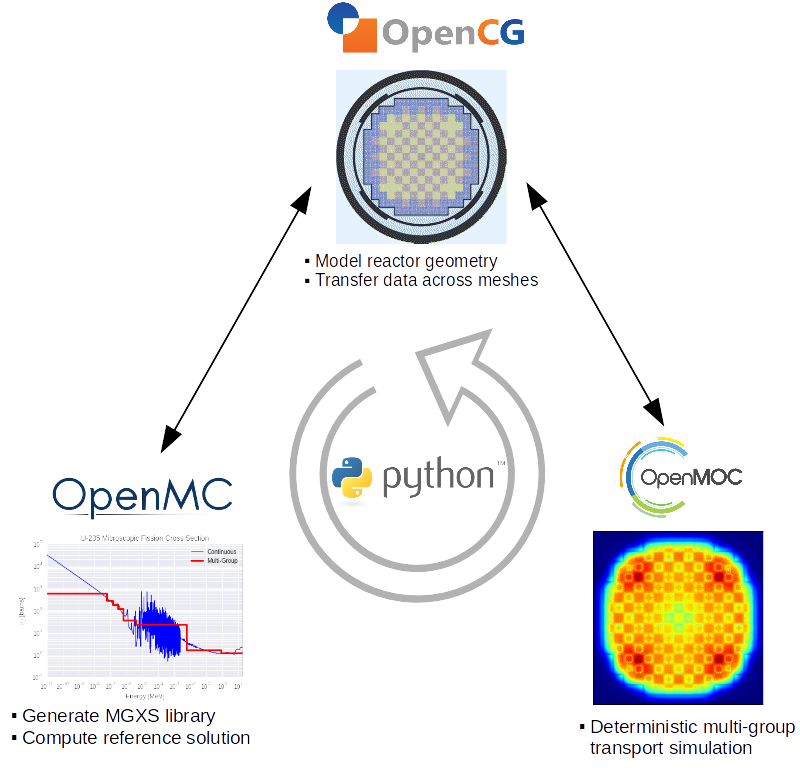
\includegraphics[width=0.8\linewidth]{figures/workflow/simulation-triad}
\caption[A simulation triad of OpenMC, OpenMOC and OpenCG]{A simulation triad consisting of the OpenMC, OpenMOC and OpenCG codes ``glued'' together with Python formed the foundation for this thesis research.}
\label{fig:chap4-simulation-triad}
\end{figure}

This thesis developed new features for the OpenMC code to enable the processing of large tally datasets to generate \ac{MGXS}. These contributions were motivated by the novel spatial homogenization technique presented in Chap.~\ref{chap:unsupervised} which requires the calculation of microscopic \ac{MGXS} for each nuclide in each spatial zone across a reactor core geometry. The tally datasets for this scheme are orders of magnitude larger than those generated by the multi-level approaches previously considered in the literature. In particular, the tally datasets are computed on a fine (\textit{e.g.}, pin-wise) spatial tally mesh for a fully-detailed heterogeneous whole-core geometry. This stands in contrast to multi-level approaches which compute \ac{MGXS} for each unique fuel pin or assembly with infinite lattice boundary conditions for use in a multi-group whole-core calculation. For example, the scheme introduced here would tally \ac{MGXS} for each of the 50,000+ fuel pins in a whole-core \ac{PWR} \ac{MC} simulation. In contrast, a multi-level approach would compute \ac{MGXS} for the 10s of unique fuel pins or assemblies in the model with pin-wise or assembly-wise \ac{MC} simulations.

This thesis' requirements for ``big data'' Monte Carlo calculations can be defined along two primary dimensions: scalable parallel algorithms for efficient \ac{MC} tracking, sampling and tallying, along with flexible and robust tools for downstream data processing. The first of these dimensions has been a focal point for OpenMC development since its inception. OpenMC includes distributed memory parallelism via the Message Passing Interface (MPI) and has been shown to scale with near perfect efficiency to 100,000s of processor cores~\cite{romano2013parallel}. In addition, shared memory parallelism is implemented with the OpenMP library~\cite{siegel2014multi} which reduces the simulation memory footprint by minimizing domain replication on multi-core processors. Furthermore, recent work has developed innovative schemes to manage tally datasets with memory footprints beyond that available on a single node in a typical \ac{HPC} machine (a few tens of gigabytes) with tally servers~\cite{romano2013servers} and spatial domain decomposition~\cite{horelik2014dd}. The efficient parallel algorithms already implemented in OpenMC were a key reason to use the code for this thesis work.

However, this thesis did involve the development of software tools to address the data processing needs for ``big data'' \ac{MC} calculations. It is the author's opinion that these data processing tools address uniquely position OpenMC as the only \ac{MC} code presently capable of supporting the \ac{MGXS} generation scheme introduced in this thesis. For example, many commonly \ac{MC} codes store and retrieve tally data from \ac{ASCII} formatted files or flat binary files. Although these file formats may work well for small tally datasets, they do not scale well for the tally datasets used in this thesis. The data processing paradigm reinforced by many \ac{MC} codes places an large burden on the user to write convoluted parsers to extract tally data without a generic set of tools to guide the process. In addition, many tally data stores are organized in a way that necessarily serializes tally data access without the metadata needed to index data in an efficient and parallel manner. Furthermore, many data stores are highly tailored to tallies on Cartesian or hexagonal meshes rather than the more complex unstructured meshes needed to generate \ac{MGXS} for fine mesh transport codes. The software tools developed for this thesis attempt to mitigate these issues and formalize a flexible and scalable tally data model for OpenMC.

%The development of a next-generation data model for OpenMC took a user-centric approach with the following three focus areas:

%\begin{itemize}[noitemsep]
%\item \textbf{Expressive Input} -- intuitive and compact simulation model descriptions
%\item \textbf{Managed Execution} -- automated optimization of simulation performance
%\item \textbf{Seamless Processing} -- scalable tools to index and transform tally data
%\end{itemize}

This section describes the features introduced to develop the next-generation model in OpenMC and follows a recent paper by this author~\cite{boyd2016bigdata}. Sec.~\ref{sec:chap3-py-api} presents a fully-featured Python \ac{API} for OpenMC which formed the foundation for much of this work. An algorithm to simplify tally management on unstructured but repeated tally volumes is highlighted in Sec.~\ref{sec:chap3-distribcells}. Finally, a new module to generate \ac{MGXS} was implemented atop many of the newly introduced features in OpenMC as discussed in Sec.~\ref{sec:chap3-mgxs}. All of the feature implementations were peer reviewed and incorporated into the v0.7.1 release of OpenMC.

%%%%%%%%%%%%%%%%%%%%%%%
\subsection{Python API}
\label{sec:chap3-py-api}

A fully-featured Python \ac{API} was designed and implemented to enable programmatic pre- and post-processing for OpenMC~\cite{boyd2016bigdata}. The \ac{API} enables tight coupling of input generation, simulation execution, and tally data analysis within dynamic Python script ``input files.'' In addition, the \ac{API} makes it possible to leverage the extensive ecosystem of Python packages for scientific computing alongside OpenMC in a simulation workflow. The following sections describe the \ac{API} and some of the core features which form the basis of the software stack developed to support the \ac{MGXS} generation module created for OpenMC.

%%%%%%%%%%%%%%%%%%%%%%%%%%%%%%%%%
\subsubsection{Overview}
\label{sec:chap3-py-api-overview}

%-important to have flexible handle on the geometry for high-fidelity spatial tallies

The Python \ac{API} is a user-friendly, complementary (and optional) addition to the OpenMC codebase. OpenMC is written in Fortran 2008 and uses \ac{XML} input files to describe the simulation materials, geometry, tallies, and settings. Although \ac{XML} is often hailed as both human-readable and machine-readable, it is cumbersome to write by hand for large and complicated reactor models such as those modeled in this thesis. The Python \ac{API} circumvents this process by leveraging Python's internal \texttt{ElementTree} \ac{API} to generate the \ac{XML} files used by the OpenMC executable. Instead of writing \ac{XML} files by hand, dynamic Python scripts are used to describe one or more OpenMC simulations, including those used to generate \ac{MGXS} with OpenMC.

The OpenMC Python \ac{API} adheres to object-oriented software design principles with extensible class definitions. A user instantiates, manipulates, and connects objects representing items such as cells, materials, and tallies to construct an OpenMC simulation. This is a scalable alternative workflow to traditional ``decks'' of ``cards'' in which data characterizing a simulation is specified in opaque \ac{ASCII} files (\textit{e.g.}, integer identifiers for cells, materials, and tallies). The Python \ac{API} provides classes and routines to represent all features provided by OpenMC's \ac{XML} input specifications.

In addition to its functionality for input generation, the Python \ac{API} also includes a rich framework of tally data processing utilities. The \ac{API} eliminates the time intensive and error prone process of writing code to parse results from OpenMC's output files. The \ac{API} is able to reconstruct the hierarchy of interconnected Python objects used to represent the materials, geometry and tallies from OpenMC's ``statepoint'' and ``summary'' \ac{HDF5} output files~\cite{koranne2011hdf5}. OpenMC's dynamic object-oriented data processing model -- fusing the geometry and materials configuration with tallied data -- enabled the rapid calculation, indexing and storage of \ac{MGXS} from tallies on unstructured meshes for this thesis.
  
%%%%%%%%%%%%%%%%%%%%%%%%%%%%%%%%%
\subsubsection{Pandas DataFrames}
\label{sec:chap3-pandas-df}

The Python API encapsulates numerical tally data using $N$-dimensional array objects from the NumPy package~\cite{walt2011numpy}. Although OpenMC's NumPy interface to tally data is more flexible than simply reporting the data in \ac{ASCII} files, NumPy arrays are relatively opaque containers for managing large tally datasets. A single OpenMC \texttt{Tally} object used for \ac{MGXS} generation may encompass many different energy groups, nuclides and reaction types, yet all of this data is tabulated in a single contiguous NumPy array. As a result, it is challenging to implement general algorithms to index, inspect and manipulate tally data in NumPy arrays for specific groups, nuclides or reactions.

The Pandas Python package~\cite{mckinney2010pandas} was implemented in the Python \ac{API} to enable transparent tally data processing for \ac{MGXS} generation. In particular, the \texttt{Tally} class includes a feature to construct a Pandas 
\texttt{DataFrame} object from tally data. Pandas \texttt{DataFrames} are modeled after data structures in the \textsf{R} programming language used to store data tables in a more accessible format than contiguous arrays. Pandas \texttt{DataFrames} support mixed-type data (\textit{i.e.}, strings and numbers), and allow the use of string keys or labels to index each column or row. The Python \ac{API} uses this capability to build Pandas DataFrames by annotating tally data with the filters, nuclides, and scores associated with each tally bin. 

Pandas' most advanced features are intended for scalable data manipulation operations such as sorting, merging, and joining datasets, and generating pivot tables. In addition, Python's powerful statistics and machine learning packages -- such as SciPy~\cite{jones2011scipy}, statsmodels~\cite{seabold2010statsmodels} and scikit-learn~\cite{pedregosa2011sklearn} -- are well integrated with Pandas and may be easily applied to \texttt{DataFrames} of tally data. Pandas \texttt{DataFrames} were extensively used to encapsulate tally data throughout the statistical data processing framework for the \ac{MGXS} spatial homogenization methology introduced in this thesis.

%%%%%%%%%%%%%%%%%%%%%%%%%%%%%%%%
\subsubsection{Tally Slicing and Merging}
\label{sec:chap3-tally-slice-merge}

Two useful and related features in the OpenMC Python \ac{API} for \ac{MGXS} generation are \textit{tally merging} and \textit{tally slicing} as depicted in Fig.~\ref{fig:tally-merge-slice}. Although it is useful to systematically create individual \texttt{Tally} objects for each spatial zone and reaction type when generating the OpenMC inputs necessary to compute \ac{MGXS}, which leads to a large number (10$^2$ -- 10$^3$) of tallies objects for large, complex geometries. The large number of distinct tallies poses a computational bottleneck since the overhead to tally in OpenMC scales as $\mathcal{O}(N)$ for $N$ tallies. To compensate for this, the Python \ac{API}'s \texttt{Tally} class allow for the automated merging of tallies for input generation. Similarly, the \ac{API} supports the slicing of tallies to simplify downstream data processing which may comprise energy-, nuclide-, and/or reaction-dependent transformations of the tally data. Tally merging and slicing are extensively used throughout the statistical data processing framework for the \ac{MGXS} spatial homogenization methology introduced in this thesis.

\begin{figure}
\begin{subfigure}{\textwidth}
  \centering
  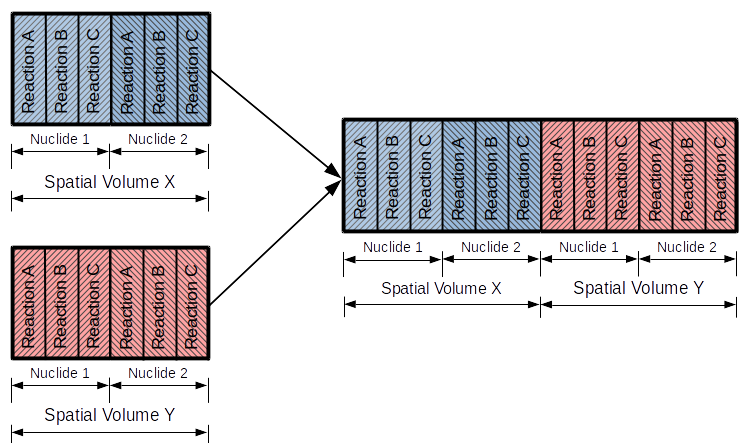
\includegraphics[width=\linewidth]{figures/workflow/tally-merge}
  \caption{}
\end{subfigure}
\begin{subfigure}{\textwidth}
  \centering
  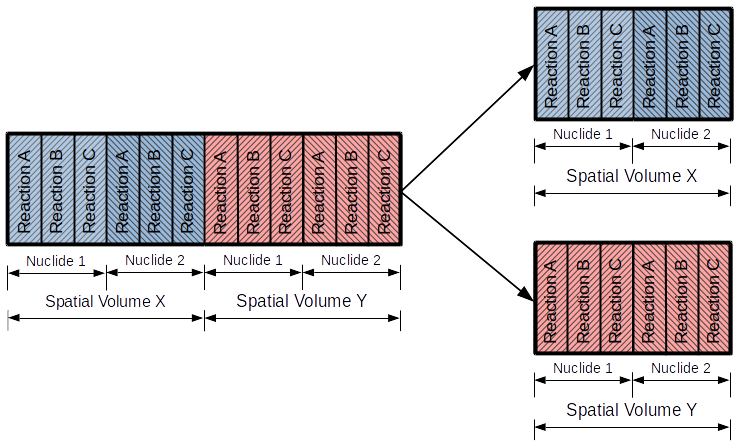
\includegraphics[width=\linewidth]{figures/workflow/tally-slice}
  \caption{}
\end{subfigure}
\caption[Tally merging and slicing operations]{Two \texttt{Tally} objects for different spatial volumes are merged into a single \texttt{Tally} (a). A single \texttt{Tally} is sliced by tally volume into two distinct \texttt{Tally} objects (b).}
\label{fig:tally-merge-slice}
\end{figure}

%paragraph: aggregation (slicing/merging)
%-operations use NumPy to efficiently create derived sliced/merged tallies
%-slicing/merging can be used to slice tallies apart by nuclide, group, domain, etc.
%  -use tally merging to re-assembly MGXS from outputs of ML algorithms

%%%%%%%%%%%%%%%%%%%%%%%%%%%%%%%%
\subsubsection{Tally Arithmetic}
\label{sec:chap3-tally-arithmetic}

As discussed in Sec.~\ref{subsec:chap3-tally-types}, a variety of reaction rate and flux tallies must be arithmetically combined in order to compute \ac{MGXS} with Monte Carlo. At the most general level, a reaction rate tally must be divided by a flux tally for each energy group, nuclide and tally volume (see Eqn.~\ref{eqn:chap3-general-micro}). In addition, the transport correction must be subtracted from the total cross section and scattering matrix, and a summation must be performed over energy groups to compute the fission emission spectrum. Furthermore, it is desirable to compute an estimate of the uncertainty for each \ac{MGXS} by propagating uncertainties as described in Sec.~\ref{subsec:chap3-uncertainty-prop}. The Python \ac{API} provides a novel feature known as \textit{tally arithmetic} to enable arithmetic combinations of tallies with efficient vectorized numerical operations across energy groups, nuclides and spatial tally zones.

Tally arithmetic is an object-oriented data processing feature which arithmetically combines two or more tallies and/or scalar values into new ``derived tallies.'' The objective of tally arithmetic is to rapidly transform tally data with automated uncertainty propagation. The tally arithmetic implementation in OpenMC overloads the operators for addition, subtraction, multiplication, division, and exponentiation in the Python \ac{API}'s \texttt{Tally} class. In addition, the \texttt{Tally} class supports summation or averaging operations across some or all its filter, nuclide or score bins.  The derived tallies created by tally arithmetic provide with the same rich functionality available for the \texttt{Tally} operands used in the arithmetic operation (\textit{e.g.}, Pandas DataFrames).

Multi-group cross sections are simply and efficiently computed with tally arithmetic. For example, the following code snippet illustrates how tally slicing and arithmetic are used to compute a total \ac{MGXS}:

\lstinputlisting[language=Python, basicstyle=\ttfamily\footnotesize, caption={\ac{MGXS} calculation with tally arithmetic.}, label={lst:python-input}]{listings/workflow/tally-arithmetic.py}

\noindent The total \ac{MGXS} that is returned from the tally division operation is encapsulated within a \texttt{Tally} class. This is the approach used by the \ac{MGXS} generation module created for OpenMC in Sec.~\ref{sec:chap3-mgxs}.

It should be noted that the uncertainty propagation in tally arithmetic makes the assumption that tallies represent independent random variables (see Sec.~\ref{subsec:chap3-uncertainty-prop}). However, in many if not most cases this assumption is untrue as tallies may be highly correlated. For example, there is a strong correlation between the flux and reaction rate tallies across the same material or cell, but this is not accounted for when these tallies are combined to compute \ac{MGXS} with tally arithmetic. In the future it may be possible to improve this approximation with the inclusion of tally covariance matrices in tally arithmetic.

%%%%%%%%%%%%%%%%%%%%%%%%%%%%%%%%%%%%%
\subsection{Distributed Cell Tallies}
\label{sec:chap3-distribcells}

first paragraph: motivation
-

second paragraph: combinatorial geometry
-pros vs. cons

third paragraph: distribcell algorithm
-overview algorithm
-look at PHYSOR 2014 paper
-

fourth paragraph:
-advantages of algorithm
  -single line of \ac{XML} code
  -no need to change the geometry
  -vectorized operations with Python API
-potential disadvantages?
  -quite complex to think through
  -tough to debug

fourth paragraph: tie back to MGXS
-need MGXS in each tally zone 
-

\begin{itemize}
  \item Capture \ac{MGXS} spatial variation~\cite{lax2014distribcell}
\end{itemize}

\begin{figure}
    \centering
    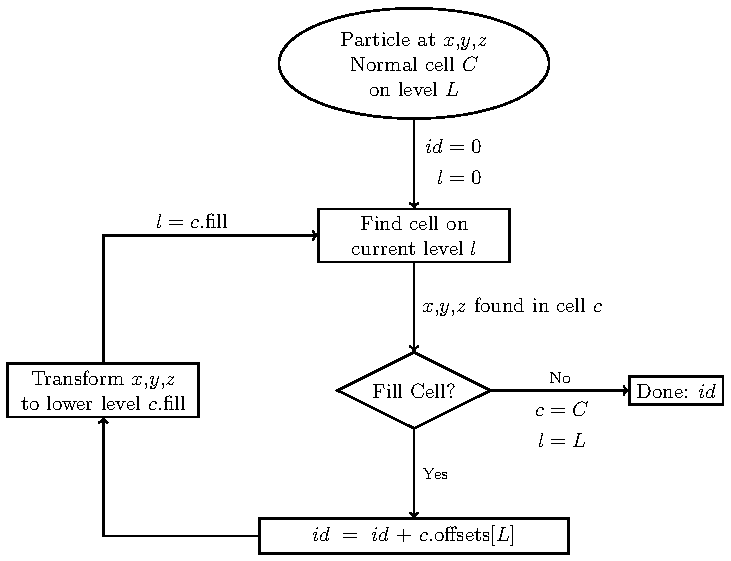
\includegraphics[width=6in]{figures/workflow/openmc/flow.pdf}
    \caption{\label{fig:indexing_scheme} Example geometry with 3 universe levels.  Material cells are defined in pin-cell universes $a$ and $b$, which are filled into the cells of lattice universes $B$ and $C$, which are filled into the cells of lattice universe $A$.  The colored numbers in each fill cell are the offsets for each base universe, which can be used to quickly compute a unique ID for each instance of a material cell.}
\end{figure}

\begin{figure}[htb!]
    \centering
    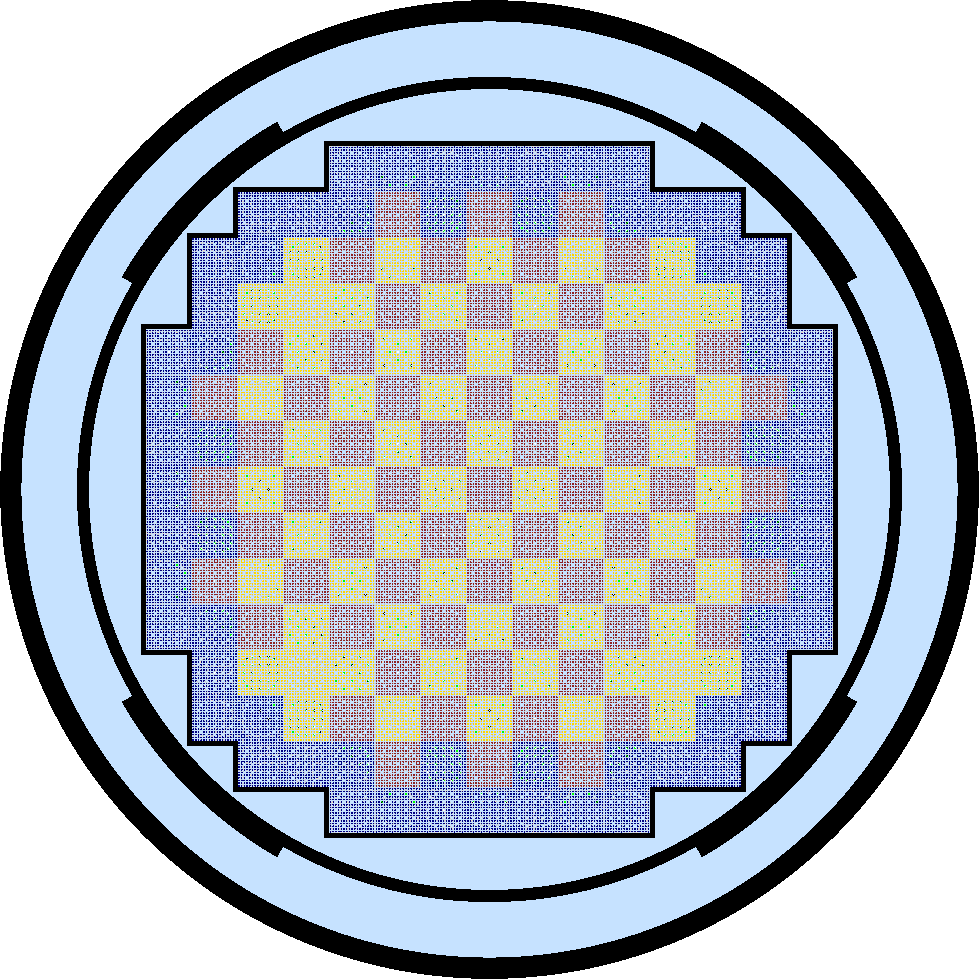
\includegraphics[width=2in]{figures/workflow/openmc/core}\hspace{1cm}
    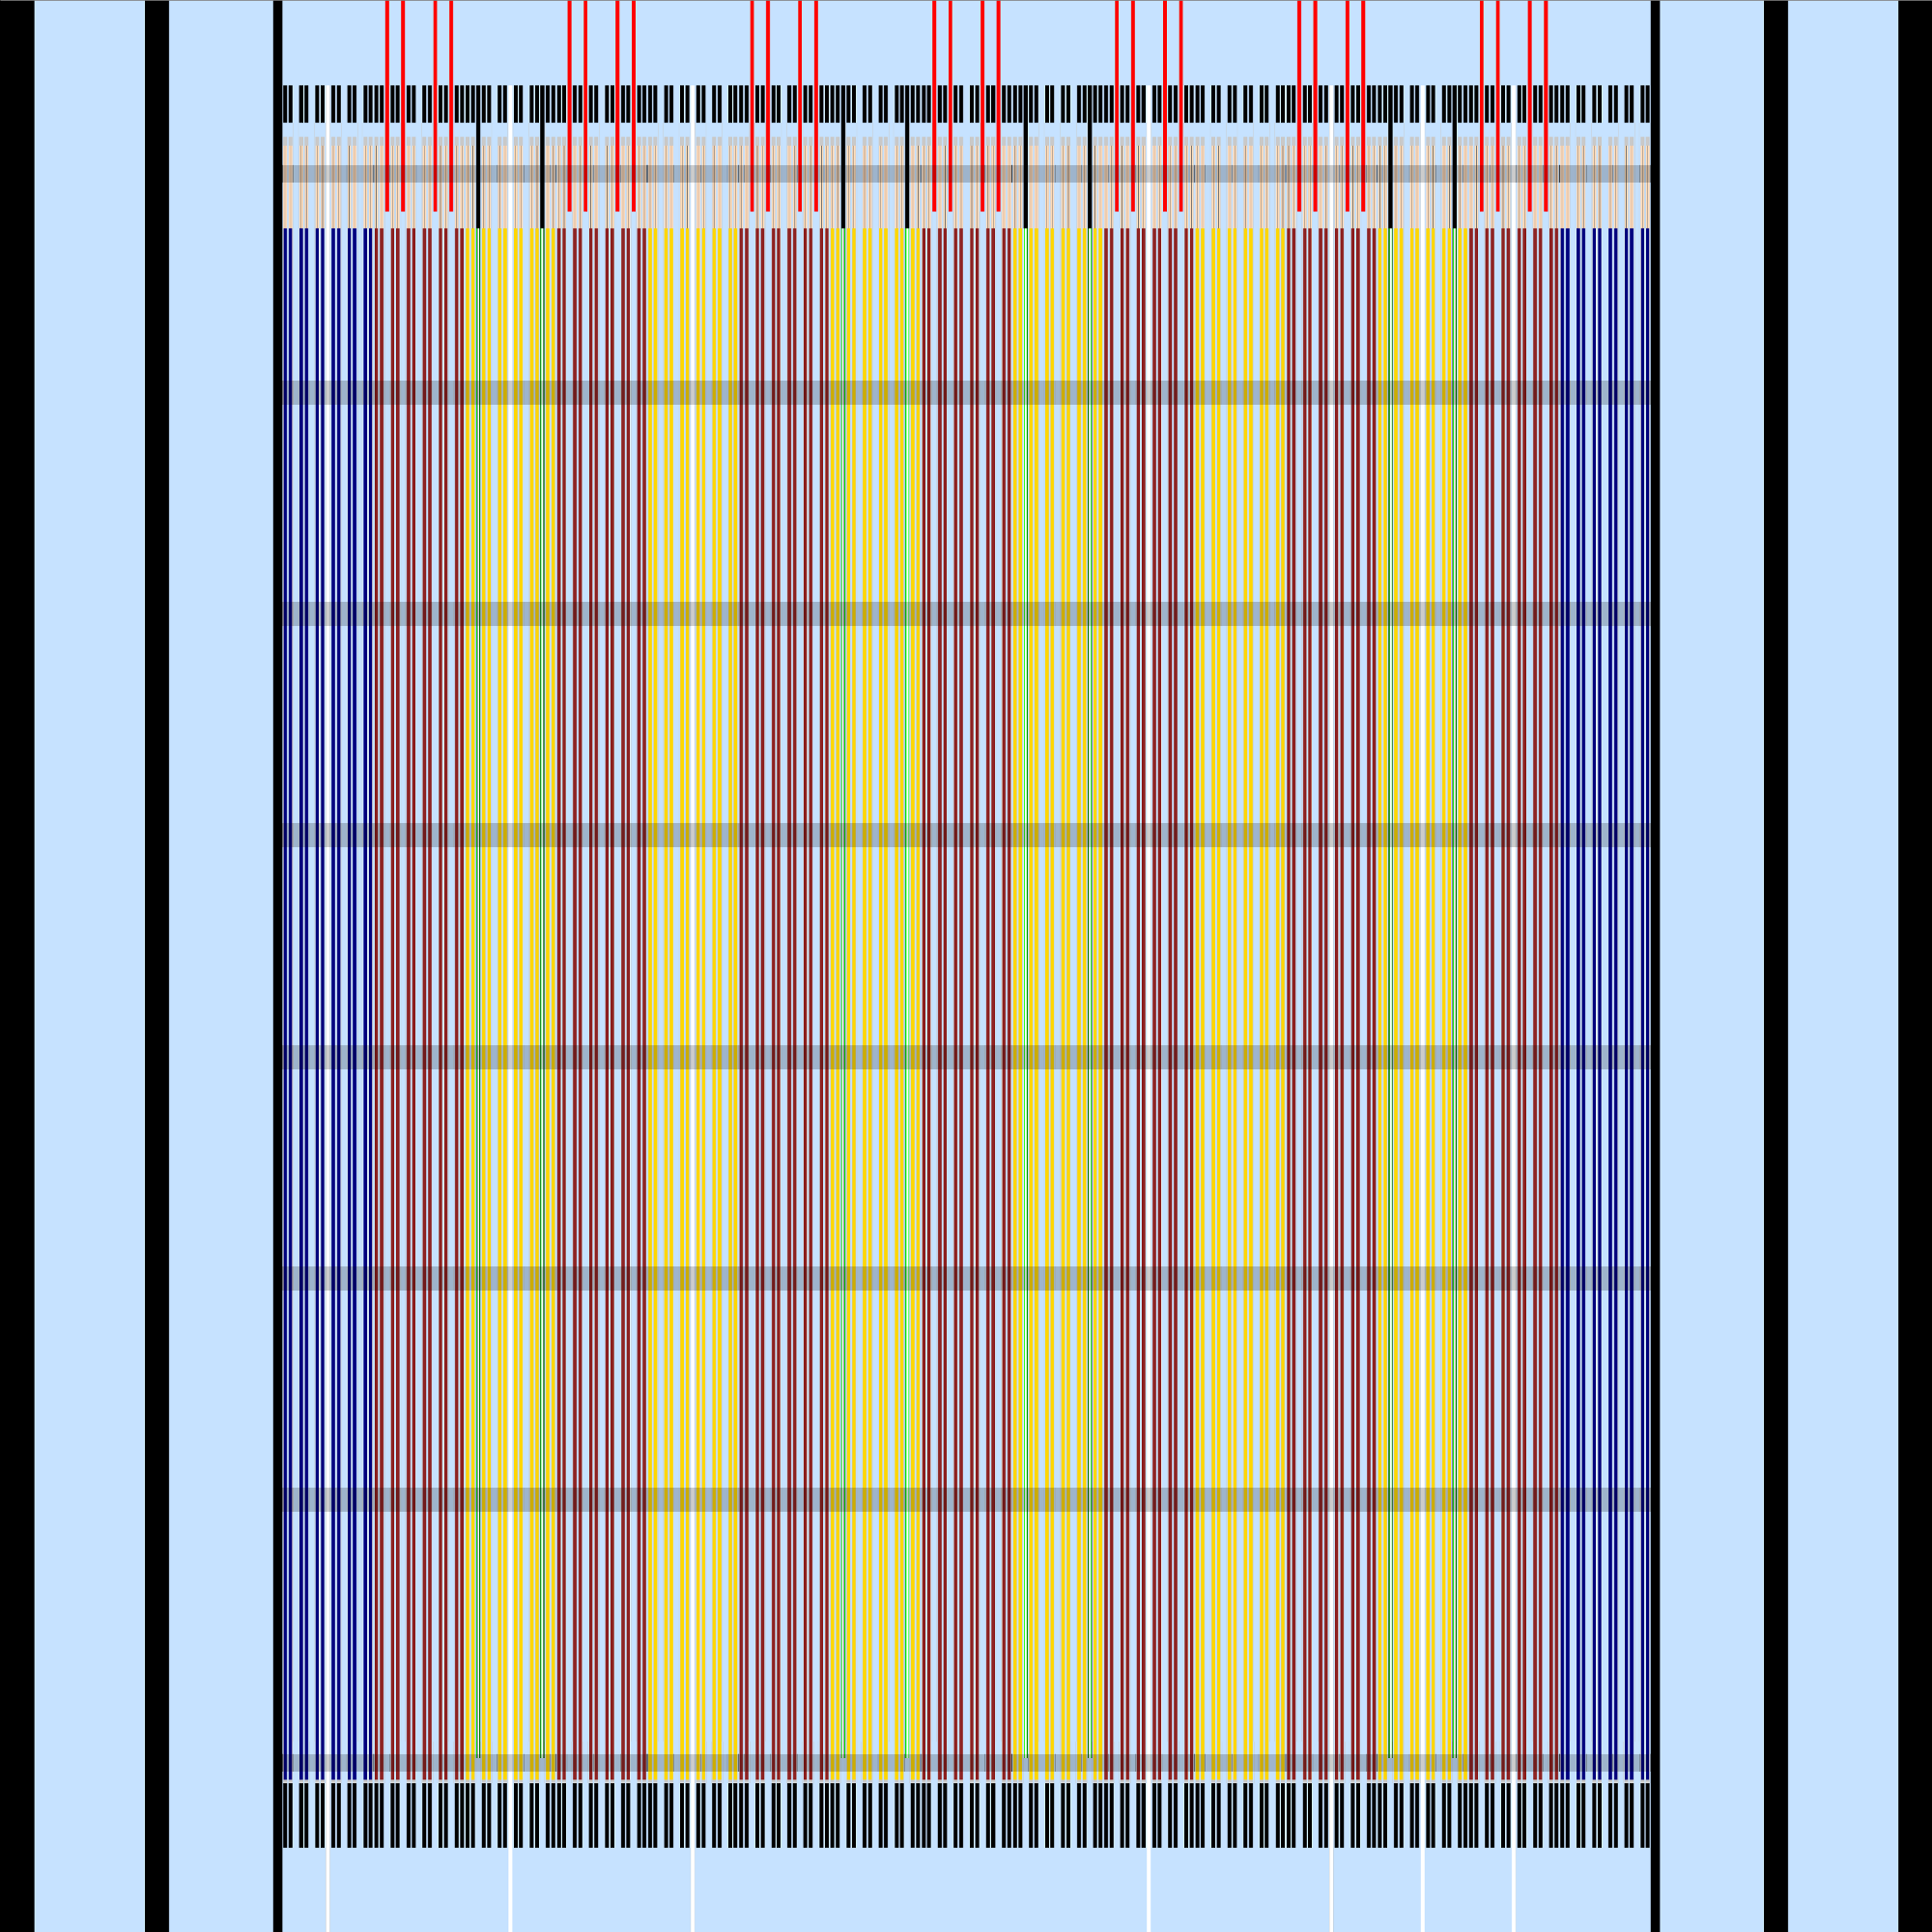
\includegraphics[width=2in]{figures/workflow/openmc/core_axial}
    \caption{\label{fig:beavrs} Geometry of the BEAVRS benchmark. \emph{Left:} Radial view, showing 193 fuel assemblies, colored by enrichment. \emph{Right:} Axial view, showing grid spacers and axial pin-cell features.}
\end{figure}

%%%%%%%%%%%%%%%%%%%%%%%%%%%%
\subsection{MGXS Generation}
\label{sec:chap3-mgxs}

\begin{itemize}[noitemsep]
  \item Python \ac{API} software stacks together in \texttt{openmc.mgxs}
\end{itemize}

-perhaps a figure with 

%%%%%%%%%%%%%%%%%%%%%%%%%%%%%%%%%%%%%%%%
\subsection{Isotropic-in-Lab Scattering}
\label{sec:chap3-iso-in-lab}


%%%%%%%%%%%%%%%%%%%%%%%%%%%%%%%%%%%%%%%%%%%%%%%%%%%%%%%%%%%%%%%%%%%%%%%%%%%%%%%%
\section{OpenMOC}
\label{sec:chap3-openmoc}

\begin{itemize}[noitemsep]
  \item reference Annals paper~\cite{boyd2014openmoc}
  \item multi-core CPUs~\cite{boyd2016parallel} and GPUs~\cite{boyd2013massively}
  \item reference 3D \ac{MOC} papers
  \item brief description of \ac{MOC} equations
  \begin{itemize}[noitemsep]
    \item flat/linear source approx.
    \item isotropic approx.
    \item constant-in-angle \ac{MGXS}
    \item uses total/transport, nu-fission, (nu-)scattering matrix, chi
  \end{itemize}
\end{itemize}

\begin{figure*}[ht!]
  \begin{subfigure}[htb!]{0.32\textwidth}
    \centering
    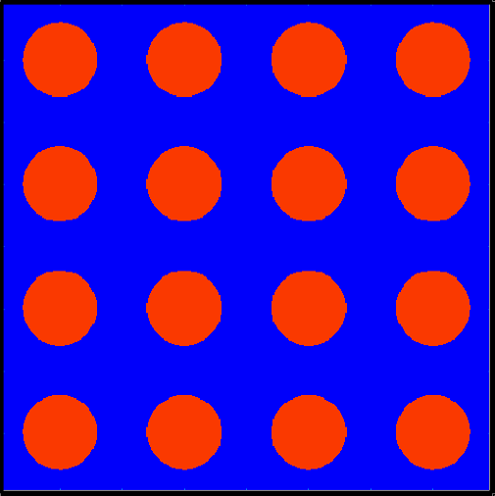
\includegraphics[width=0.95\textwidth]{figures/workflow/openmoc/materials-border}
    \label{fig:moc-model-materials}
    \caption{}
  \end{subfigure}
  \begin{subfigure}[htb!]{0.32\textwidth}
    \centering
    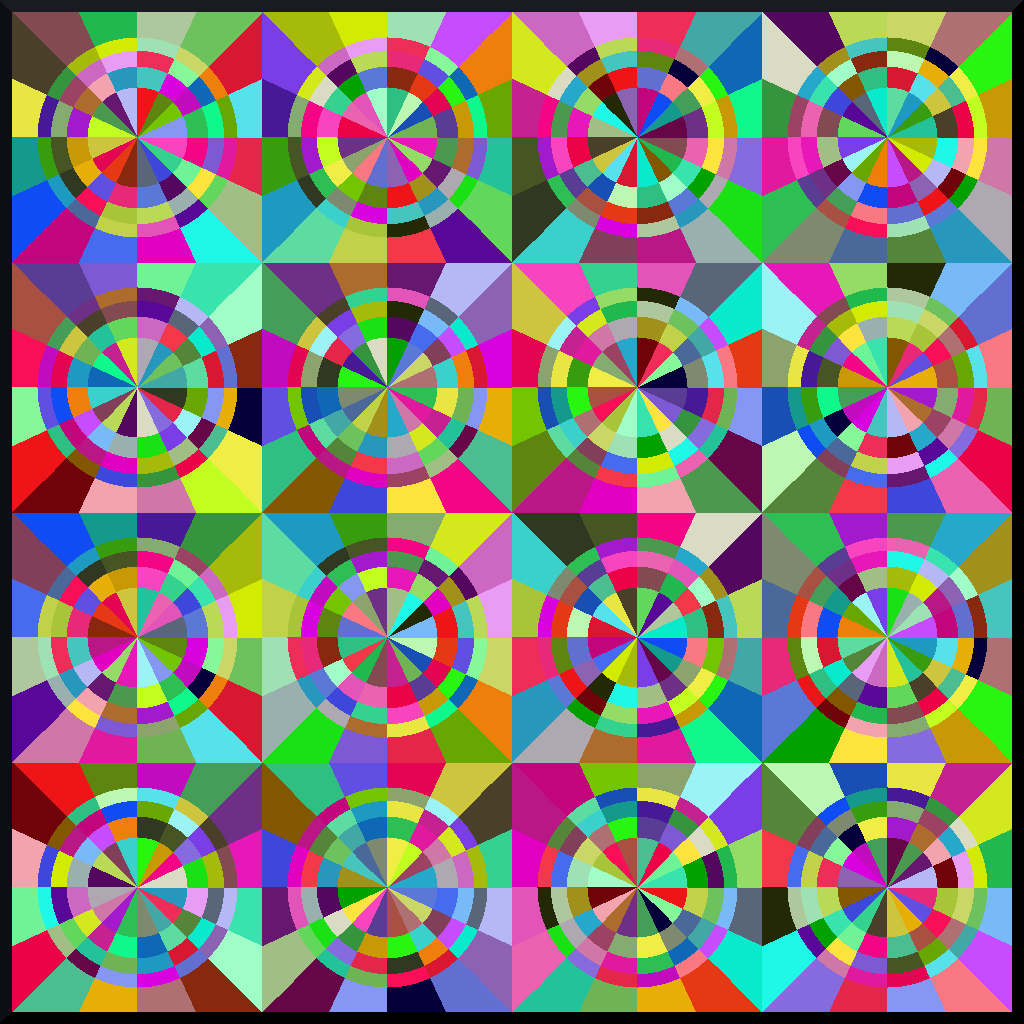
\includegraphics[width=0.95\textwidth]{figures/workflow/openmoc/FSRs}
    \label{fig:moc-model-fsrs}
    \caption{}
  \end{subfigure}
  \begin{subfigure}[htb!]{0.32\textwidth}
    \centering
    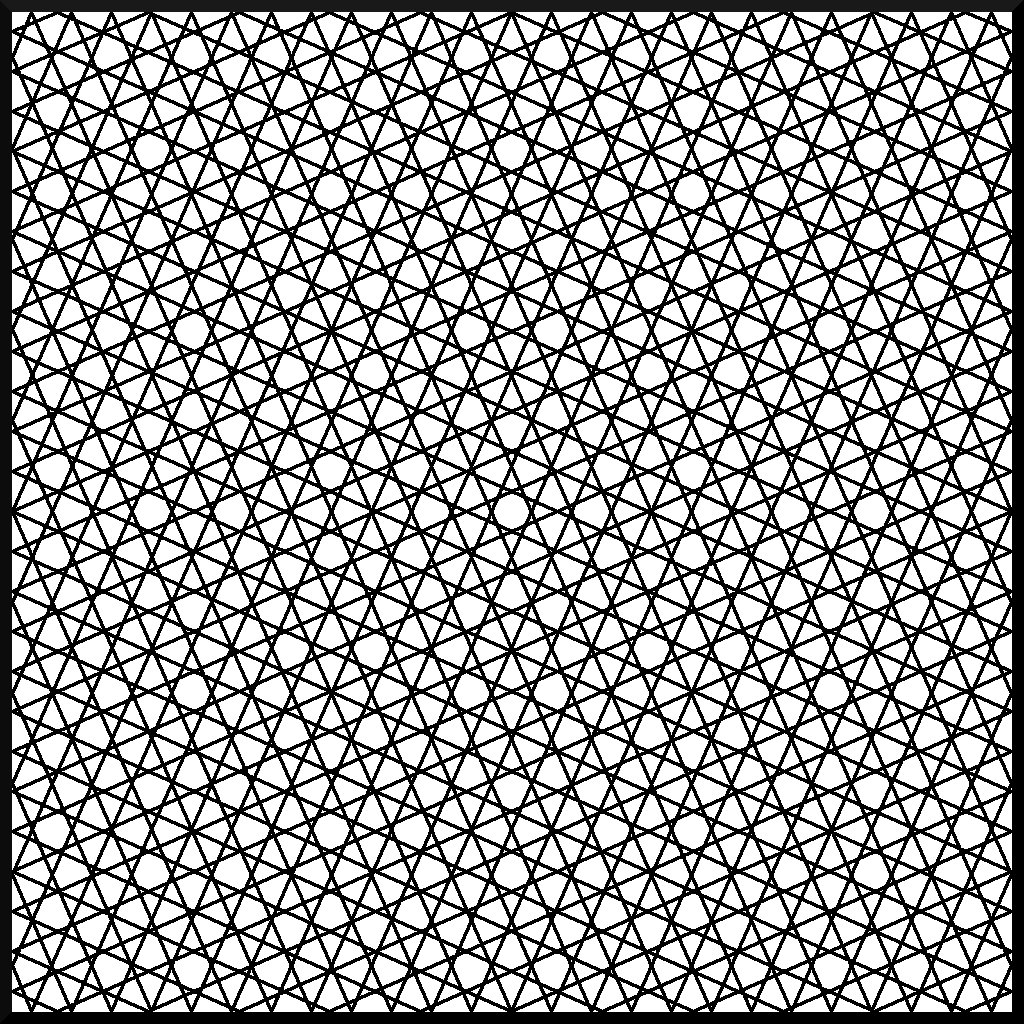
\includegraphics[width=0.95\textwidth]{figures/workflow/openmoc/cyclic-tracks}
    \label{fig:moc-model-tracks}
    \caption{}
  \end{subfigure}
\caption{The coolant and fuel materials (a), method of characteristics flat source region spatial mesh (b), and cyclic characteristic laydown (c) for a 4 $\times$ 4 fuel pin lattice.}
\label{fig:moc-model}
\end{figure*}


%%%%%%%%%%%%%%%%%%%%%%%%%%%%%%%%%%%%%%%%%%%%%%%%%%%%%%%%%%%%%%%%%%%%%%%%%%%%%%%%
\section{OpenCG}
\label{sec:chap3-opencg}

\begin{itemize}[noitemsep]
  \item single physics-agnostic geometries~\cite{boyd2015opencg}
  \item compatibility modules with OpenMC, OpenMOC
  \item ``glue'' code to map OpenMC distribcells to OpenMOC spatial mesh
\end{itemize}

\begin{figure}[h!]
  \centering
  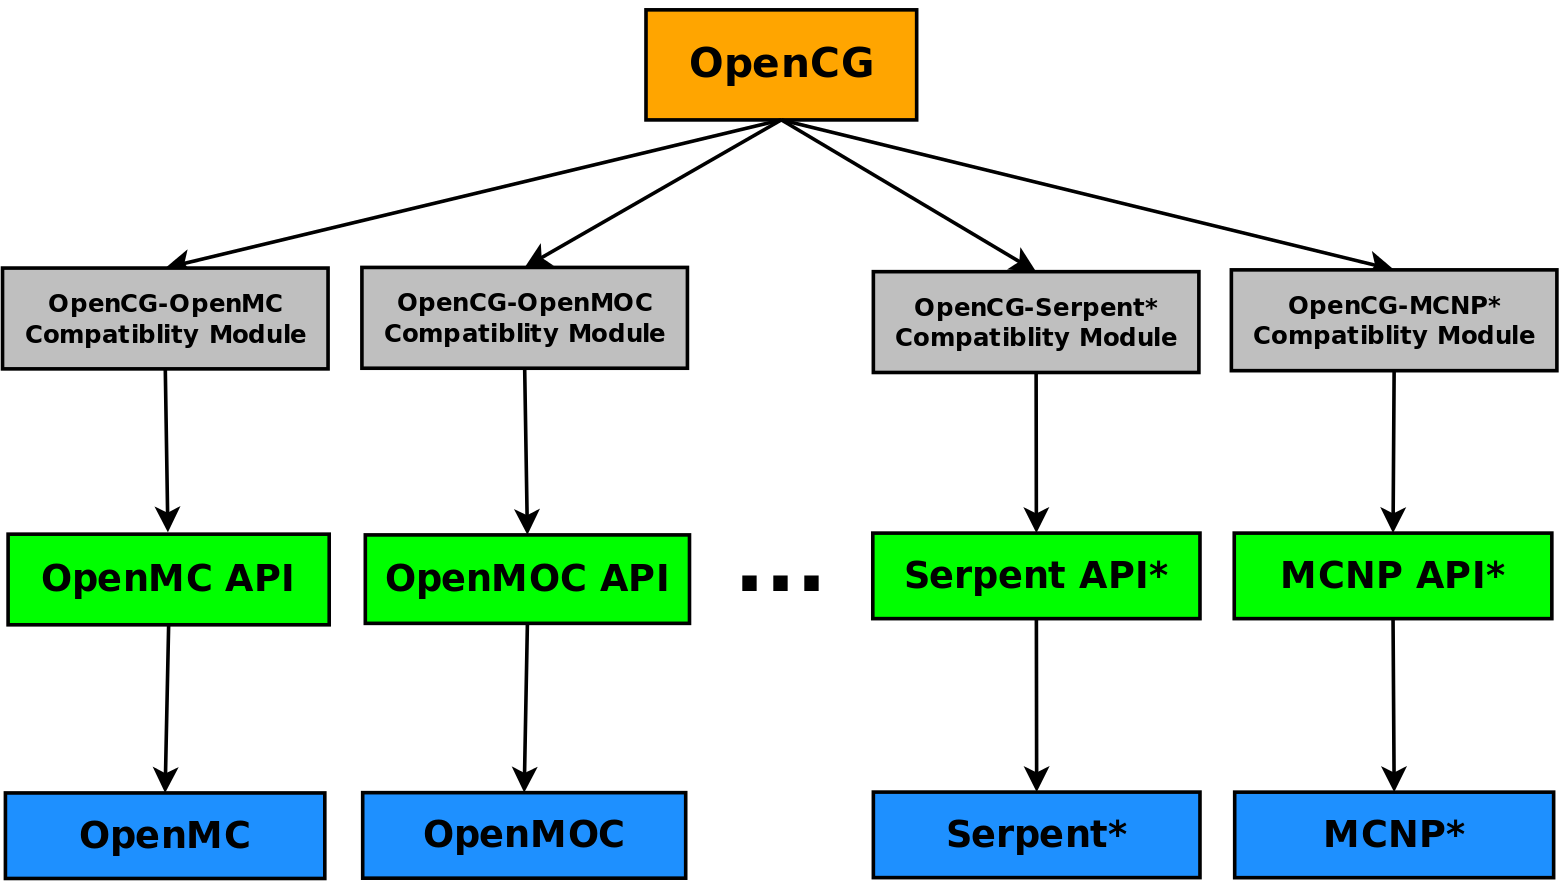
\includegraphics[width=.8\linewidth]{figures/workflow/opencg/compatibility-modules}
  \caption{OpenCG compatibility modules for various neutron transport codes. The compatibility modules for OpenMC and OpenMOC will be released in future public distributions of each code, while modules for Serpent and MCNP are in progress at the time of this writing.}
  \label{fig:compatibility-modules}
\end{figure}


%%%%%%%%%%%%%%%%%%%%%%%%%%%%%%%%%%%%
\subsection{Local Neighbor Symmetry}
\label{sec:chap3-lns}

\begin{algorithm}[h!]
\caption{Local Neighbor Symmetry Identification}
\label{alg:local-neighbor-symmetry-cells}
\begin{algorithmic}[1]
\Procedure{computeNeighborSymmetry}{$path$}
    \State $G \gets \emptyset$ \Comment{Initialize empty set for graph}
    \State $k \gets$ \textbf{length}($path$) \Comment{Find number of independent sets}
    \For{$i := 1, k$}
        \If{\textbf{type}($path[i]$) \textbf{is} UNIVERSE}
            \State $G \gets G \cup \{path[i]\}$ \Comment{Append universe to graph}
        \ElsIf{\textbf{type}($path[i]$) \textbf{is} LATTICE}
            \State $N \gets$ \Call{BreadthFirstSearch}{$path[i]$} \Comment{Find lattice cell neighbors}
            \State $G \gets G \cup \{N\}$ \Comment{Append neighbors to graph}
        \ElsIf{\textbf{type}($path[i]$) \textbf{is} CELL}
            \State $N \gets$ \Call{BreadthFirstSearch}{$path[i]$} \Comment{Find cell neighbors}
            \State $G \gets G \cup \{N\}$ \Comment{Append neighbors to graph}
        \EndIf
    \EndFor
    \State \textbf{return} \Call{Hash}{$G$} \Comment{Return $k$-partite graph hash}
\EndProcedure
\end{algorithmic}
\end{algorithm}

\begin{itemize}[noitemsep]
  \item analogy to lattice physics geometric templates based on eng. approx.
\end{itemize}

\begin{figure}
\begin{subfigure}{.5\textwidth}
  \centering
  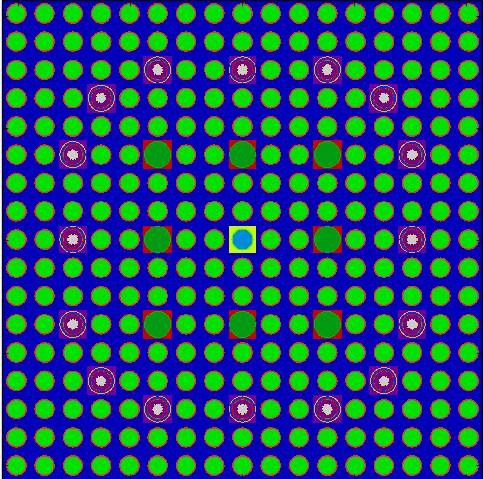
\includegraphics[width=.7\linewidth]{figures/workflow/opencg/cells-xy-24-16-assm}
  \caption{}
  \label{fig:assm-cells}
\end{subfigure}%
\begin{subfigure}{.5\textwidth}
  \centering
  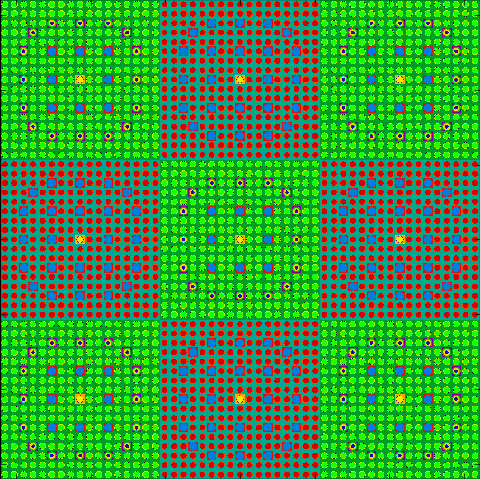
\includegraphics[width=.7\linewidth]{figures/workflow/opencg/cells-xy-colorset}
  \caption{}
  \label{fig:colorset-cells}
\end{subfigure}
\begin{subfigure}{.5\textwidth}
  \centering
  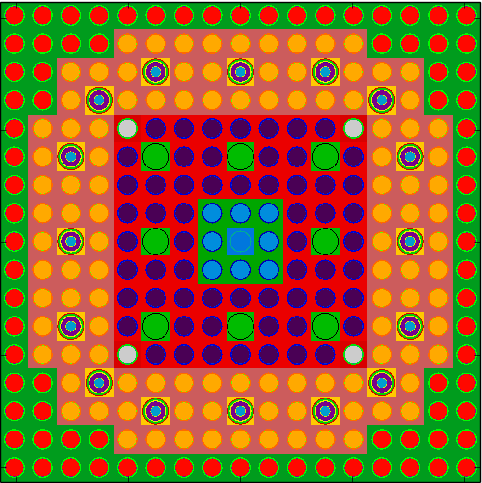
\includegraphics[width=.7\linewidth]{figures/workflow/opencg/unique-neighbor-cells-xy-24-16-assm}
  \caption{}
  \label{fig:assm-unique-neighbors}
\end{subfigure}
\begin{subfigure}{.5\textwidth}
  \centering
  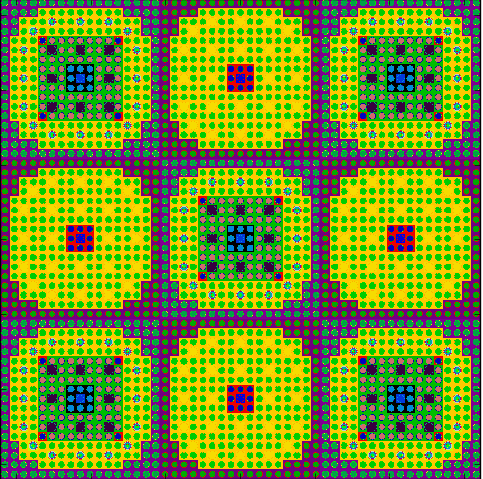
\includegraphics[width=.7\linewidth]{figures/workflow/opencg/unique-neighbor-cells-xy-colorset}
  \caption{}
  \label{fig:colorset-unique-neighbors}
\end{subfigure}
\begin{subfigure}{.5\textwidth}
  \centering
  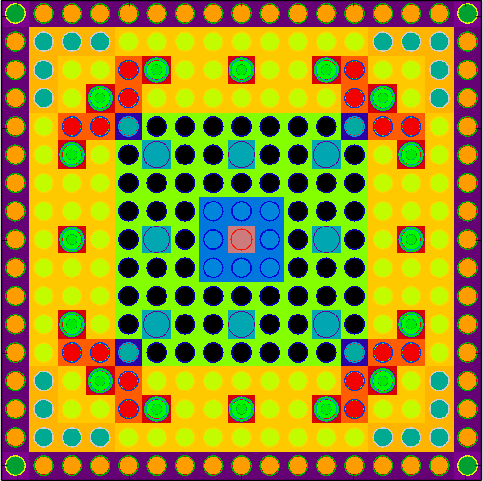
\includegraphics[width=.7\linewidth]{figures/workflow/opencg/neighbor-cells-xy-24-16-assm}
  \caption{}
  \label{fig:assm-neighbors}
\end{subfigure}
\begin{subfigure}{.5\textwidth}
  \centering
  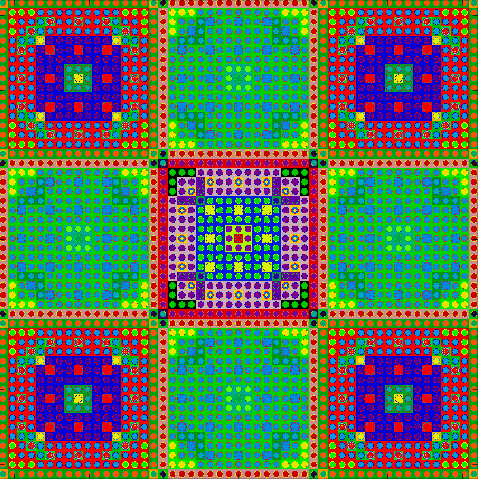
\includegraphics[width=.7\linewidth]{figures/workflow/opencg/neighbor-cells-xy-colorset}
  \caption{}
  \label{fig:colorset-neighbors}
\end{subfigure}
\caption{Two rectilinear lattice geometries are depicted to illustrate the use of local neighbor symmetry identification~\cite{boyd2015opencg}. The \textit{cells} are depicted for (a) a 17$\times$17 PWR lattice and (b) a 3$\times$3 colorset of two different 17 $\times$ 17 PWR assemblies each with burnable absorbers, guide tubes and instrument tubes. The \textit{unique neighbor} symmetry identifiers are color-coded in (c) and (d) for the assembly and colorset, respectively. Likewise, the \textit{general neighbor} symmetry identifiers are color-coded in (e) and (f).}
\label{fig:neighbor-cells}
\end{figure}

%%%%%%%%%%%%%%%%%%%%%%%%%%%%%%%%%%%%
\subsection{Region Differentiation}
\label{sec:chap3-region-diff}

\begin{itemize}[noitemsep]
  \item retain CSG's simplicity of repeated primitives for user input
  \item build combinatorial geometries based on arbitrary clustering of cell instances
\end{itemize}


\newpage
\begin{figure}[h!]
\begin{subfigure}{\textwidth}
  \centering
  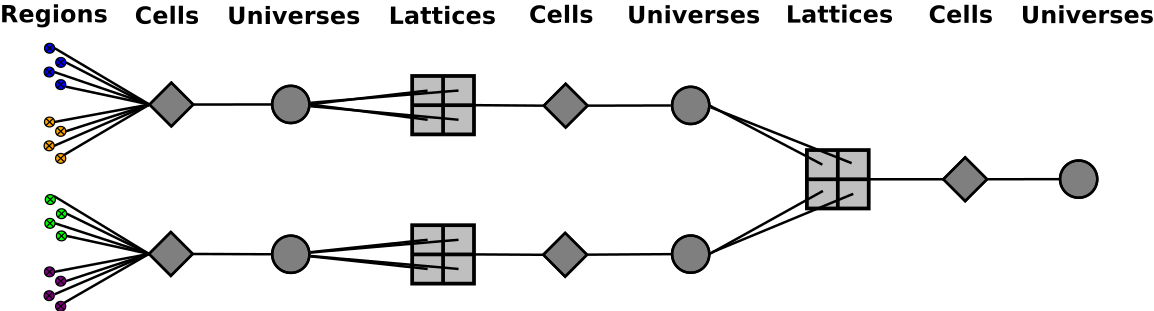
\includegraphics[width=0.82\linewidth]{figures/workflow/opencg/region-differentiation-1}
  \caption{}
  \label{fig:differentation-1}
\end{subfigure}
\begin{subfigure}{\textwidth}
  \centering
  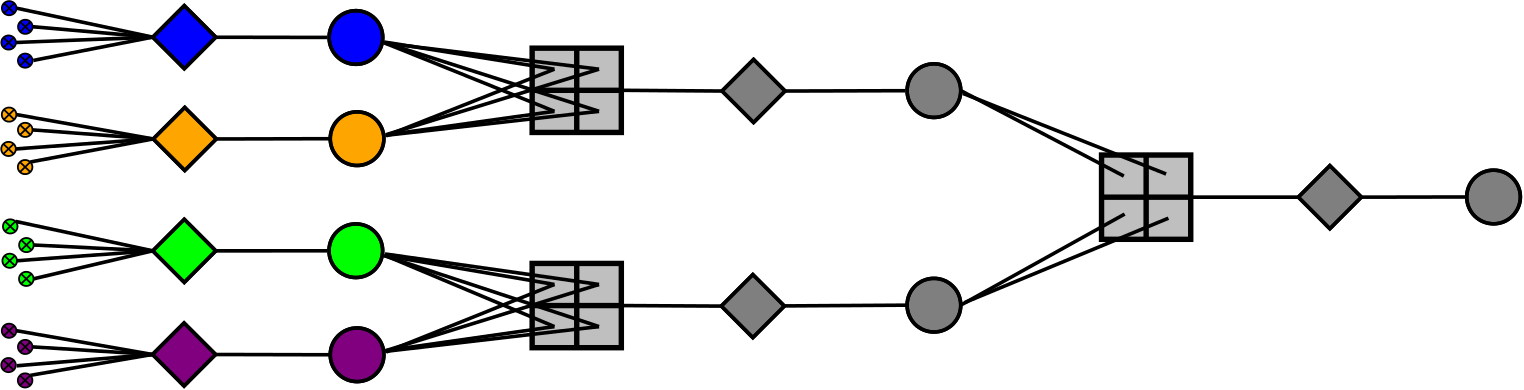
\includegraphics[width=0.75\linewidth]{figures/workflow/opencg/region-differentiation-2}
  \caption{}
  \label{fig:differentation-2}
\end{subfigure}
\begin{subfigure}{\textwidth}
  \centering
  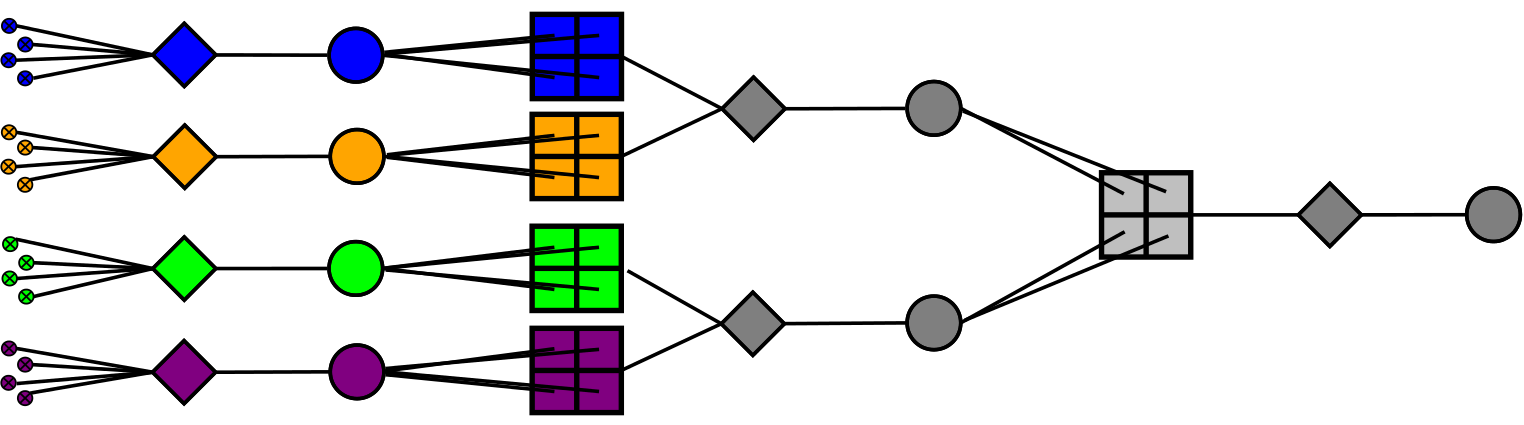
\includegraphics[width=0.75\linewidth]{figures/workflow/opencg/region-differentiation-3}
  \caption{}
  \label{fig:differentation-3}
\end{subfigure}
\begin{subfigure}{\textwidth}
  \centering
  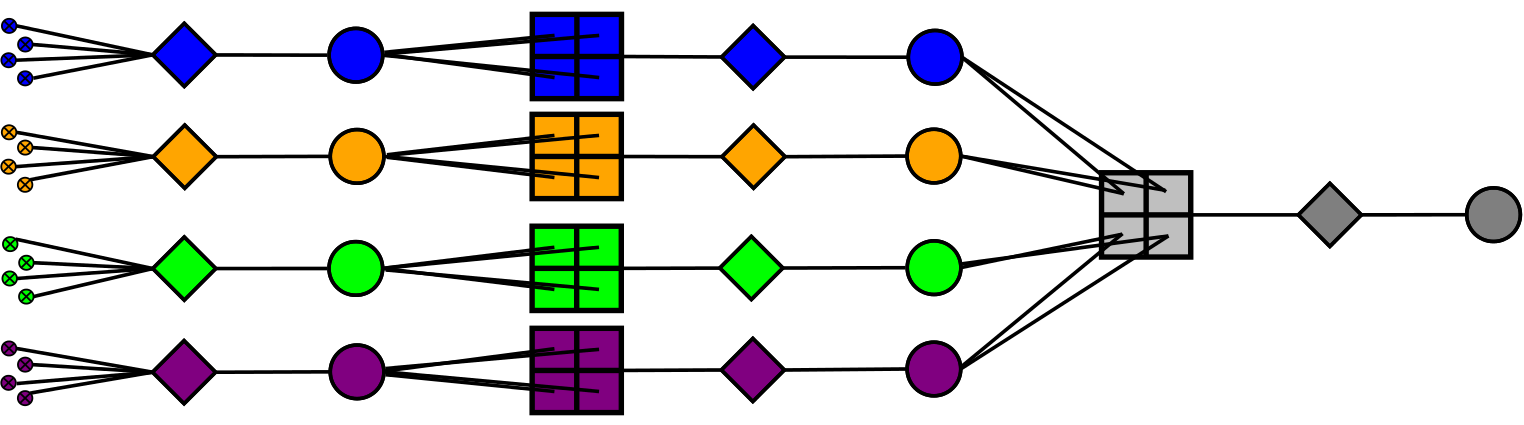
\includegraphics[width=0.75\linewidth]{figures/workflow/opencg/region-differentiation-4}
  \caption{}
  \label{fig:differentation-4}
\end{subfigure}
\begin{subfigure}{\textwidth}
  \centering
  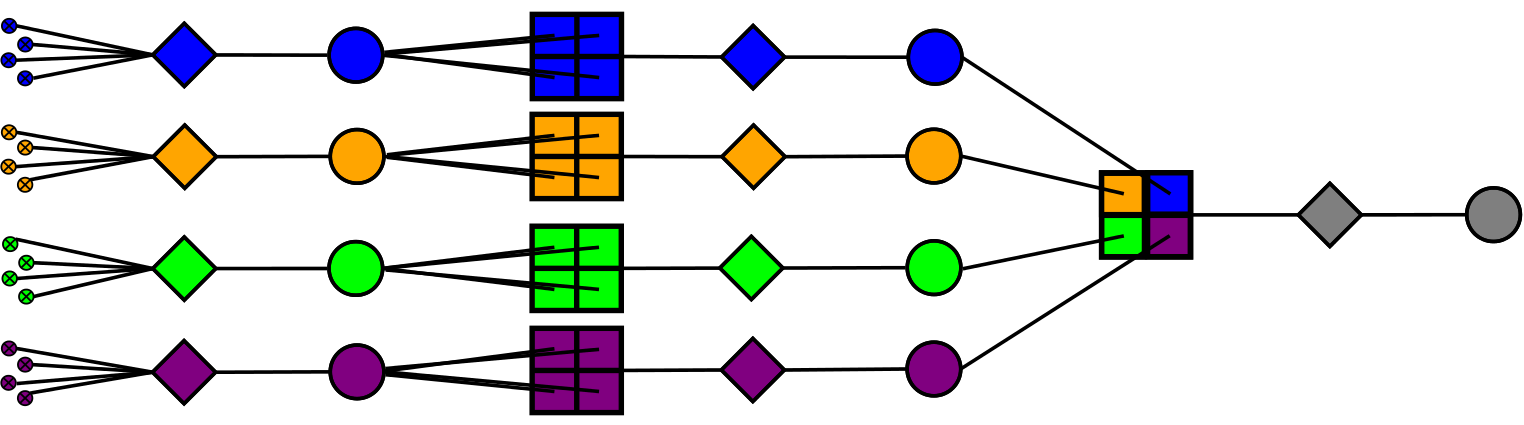
\includegraphics[width=0.75\linewidth]{figures/workflow/opencg/region-differentiation-5}
  \caption{}
  \label{fig:differentation-5}
\end{subfigure}
\caption{A few of the stages of the region differentiation algorithm~\cite{boyd2015opencg}. The regions (cell instances) to be differentiated are grouped and colored blue, orange, green and purple in (a). The first levels of cells and universes for each region group are differentiated in (b). The same is done for the lattices in (c). The algorithm continues to recursively differentiate cells, universes and lattices until no region groups collide at any level of the CG tree in (e).}
\label{fig:region-differentiation}
\end{figure}